%----------------------------------------------------------------------------------------
%    PACKAGES AND THEMES
%----------------------------------------------------------------------------------------

\documentclass[aspectratio=169,xcolor=dvipsnames]{beamer}
\usetheme{SimplePlus}

\usepackage{tikz}
\usepackage{hyperref}
\usepackage{graphicx} % Allows including images
\usepackage{booktabs} % Allows the use of \toprule, \midrule and \bottomrule in tables
\usepackage{wrapfig}
\usepackage{listings}
\usepackage[font=small,labelfont=bf]{caption}

%----------------------------------------------------------------------------------------
%    TITLE PAGE
%----------------------------------------------------------------------------------------

\title{Applying ML Methods w/ Case Study}
\subtitle{HI 743}

\author{Ryan Gallagher}

\institute
{
    Department of Health Informatics and Administration \\
    Zilber College of Public Health \\
    University of Wisconsin - Milwaukee% Your institution for the title page
}
\date{April 17th, 2025} % Date, can be changed to a custom date


%----------------------------------------------------------------------------------------
%    PRESENTATION SLIDES
%----------------------------------------------------------------------------------------

\begin{document}
\begin{frame}
    % Print the title page as the first slide
    \titlepage
\end{frame}

%----------------------------------------------------------------------------------------
%    Outline
%----------------------------------------------------------------------------------------

\begin{frame}{Overview}
    % Throughout your presentation, if you choose to use \section{} and \subsection{} commands, these will automatically be printed on this slide as an overview of your presentation
    \tableofcontents
\end{frame}

%----------------------------------------------------------------------------------------
%    Slides
%----------------------------------------------------------------------------------------

\section{The Art of Machine Learning}
\begin{frame}{The Art of Machine Learning}


\begin{itemize}
  \item Predictive analytics uses machine learning to model relationships between descriptive features and a target outcome.
  \item Machine learning adopts \textbf{inductive learning}: generalizing rules from specific instances.
  \item Inductive learning does \textbf{not guarantee truth}—rules learned from training data may not apply universally.
  \item A learning algorithm must have an \textbf{inductive bias}—a built-in assumption about the patterns to look for.
\end{itemize}
\end{frame}

\subsection{CRISP-DM / Project Structure Review}
\begin{frame}{Human Decisions in Predictive Modeling}

\begin{itemize}
  \item Learning isn't just algorithmic—\textbf{human choices shape model outcomes}.
  \item Critical decisions include:
  \begin{itemize}
    \item Feature selection and transformation
    \item Handling missing data
    \item Choice of algorithm and its parameters
    \item Evaluation and validation strategy
  \end{itemize}
  \item These choices affect:
  \begin{itemize}
    \item Model performance
    \item Interpretability
    \item Generalizability
  \end{itemize}
  \item For these reasons, machine learning is both a \textbf{science and an art}.
\end{itemize}
\end{frame}

\begin{frame}{CRISP-DM Phases and Key Questions (1/3)}

\begin{block}{\textbf{Business Understanding}}
\begin{itemize}
  \item What is the organizational problem being addressed?
  \item How can a prediction model address this problem?
  \item Do we have situational fluency?
  \item Can the organization act on the model's outputs?
  \item What data is available?
\end{itemize}
\end{block}

\vspace{0.5em}

\begin{block}{\textbf{Data Understanding}}
\begin{itemize}
  \item What is the prediction subject?
  \item What domain concepts are relevant?
  \item What is the target feature?
  \item Which descriptive features will be used?
\end{itemize}
\end{block}

\end{frame}

\begin{frame}{CRISP-DM Phases and Key Questions (2/3)}

\begin{block}{\textbf{Data Preparation}}
\begin{itemize}
  \item Are there data quality issues?
  \item How will we handle missing values?
  \item How will we normalize our features?
  \item What features will we include?
\end{itemize}
\end{block}

\vspace{0.5em}

\begin{block}{\textbf{Modeling}}
\begin{itemize}
  \item What types of models will we use?
  \item How will we set the algorithm parameters?
  \item Have underfitting or overfitting occurred?
\end{itemize}
\end{block}

\end{frame}

\begin{frame}{CRISP-DM Phases and Key Questions (3/3)}

\begin{block}{\textbf{Evaluation}}
\begin{itemize}
  \item How accurate is the model?
  \item Is the model's performance good enough to act on?
  \item Can the model's decisions be explained?
\end{itemize}
\end{block}

\vspace{0.5em}

\begin{block}{\textbf{Deployment}}
\begin{itemize}
  \item How will predictions be used in practice?
  \item How will the model be integrated into business processes?
  \item How will we monitor and maintain the model?
\end{itemize}
\end{block}

\end{frame}

\subsection{Review of Key Concepts in Predictive Modeling}
\begin{frame}{Key Concepts in Predictive Modeling}

\begin{itemize}
  \item \textbf{Target feature:} The outcome we want to predict.
  \item \textbf{Descriptive features:} Information used to make the prediction.
  \item Predictive modeling assumes a relationship exists between the target and descriptive features.
  \item We do not need to know the exact form of this relationship—just that one can be learned from data.
  \item Learning from data means \textbf{generalizing from past examples} to make future predictions.
\end{itemize}

\end{frame}

\begin{frame}{The Role of Data and Patterns in Prediction}

\begin{itemize}
  \item We learn \textbf{relationships by observing patterns} in data—this is the core of predictive analytics.
  \item These patterns allow us to build a model that makes accurate predictions on new, unseen cases.
  \item Data is used to find regularities that are \textbf{statistically consistent}, not universally true.
  \item Not all patterns are useful; some may be due to chance—\textbf{validation} is needed to confirm generalizability.
  \item Good predictive models \textbf{balance pattern detection with caution about overfitting}.
\end{itemize}

\end{frame}

\begin{frame}{The Bias-Variance Trade-Off}

\begin{itemize}
  \item A model must balance two opposing sources of error:
  \begin{itemize}
    \item \textbf{Bias:} Error from overly simplistic assumptions; leads to underfitting.
    \item \textbf{Variance:} Error from being too sensitive to the training data; leads to overfitting.
  \end{itemize}
  \item Highly complex models may capture noise as if it were signal.
  \item Very simple models may miss important patterns in the data.
  \item The goal is to find a model that's just complex enough to generalize well.
\end{itemize}

\end{frame}

\begin{frame}{Generative vs. Discriminative Approaches}

\begin{itemize}
  \item \textbf{Generative models} try to model how the data is generated.
  \begin{itemize}
    \item They capture the full joint distribution of features and outcomes.
    \item Examples include Naive Bayes and probabilistic graphical models.
  \end{itemize}

  \item \textbf{Discriminative models} focus on distinguishing between different outcomes.
  \begin{itemize}
    \item They directly learn the relationship between inputs and the target.
    \item Examples include logistic regression and decision trees.
  \end{itemize}

  \item Discriminative models often achieve higher prediction accuracy, but generative models can offer deeper insight into the data structure.
\end{itemize}

\end{frame}

\begin{frame}{Predictive vs. Explanatory Modeling}

\begin{itemize}
  \item \textbf{Explanatory models} aim to understand the underlying relationship between variables.
  \begin{itemize}
    \item Emphasis is on interpreting parameters and causal inference.
    \item Often assumes a specific form or structure to the relationship.
  \end{itemize}

  \item \textbf{Predictive models} aim to make accurate predictions on new data.
  \begin{itemize}
    \item Focus is on performance rather than interpretation.
    \item Often use flexible or complex algorithms without requiring full understanding of the underlying mechanisms.
  \end{itemize}

  \item \textbf{Key difference:} Explanatory models seek understanding, while predictive models seek accuracy.
\end{itemize}

\end{frame}


\section{Case Study: Customer Churn}


\begin{frame}
	\centering
	\Large \textbf{Case Study: Predicting Customer Churn} \\
	\vspace{.5cm}
	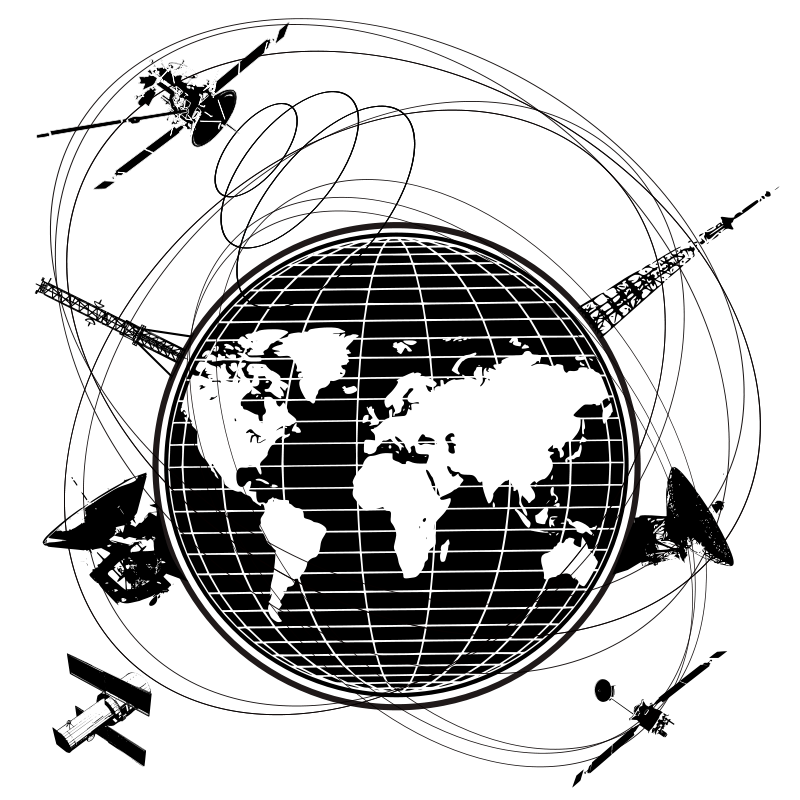
\includegraphics[scale=.2]{images/telecom.png}
\end{frame}

\begin{frame}{The Churn Problem at Acme Telephonica}

\begin{itemize}
  \item Acme Telephonica (A T) is a national mobile phone provider serving customers across all U.S. states.
  \item Like many telecom companies, A T faces a persistent challenge: \textbf{customer churn}.
  \item In 2008, A T created a customer retention team that flagged churn risks based on high volumes of support calls.
  \item These customers were offered special deals to stay—but the strategy wasn’t working.
  \item Despite efforts, churn continued to rise steadily over five years.
  \item In 2010, A T hired Ross, a \textbf{predictive analytics specialist}, to take a new data-driven approach.
  \item This case study follows Ross’s work applying the \textbf{CRISP-DM process} to build a churn prediction model.
\end{itemize}

\end{frame}
\subsection{Identify the Problem}
\begin{frame}{Understanding the Business Problem}

\begin{itemize}
  \item A T approached Ross not with a technical problem, but a \textbf{business challenge}: reducing customer churn.
  \item Ross’s first task was to translate this into a concrete analytics goal.
  \item A T aimed to reduce churn from \textbf{~10\% to 7.5\%}—a target Ross agreed was realistic, based on their data and retention strategy.
  \item Ross emphasized that model usefulness could not be confirmed until the data had been explored.
  \item He also needed to assess A T’s readiness to adopt analytics-driven decision-making and act on its insights.
\end{itemize}

\end{frame}

\begin{frame}{Understanding Operations and Data Environment}

\begin{itemize}
  \item Ross met with Kate, leader of the customer retention team, to learn about current churn interventions.
  \begin{itemize}
    \item Customers making more than 3 support calls in 2 months were flagged as churn risks.
    \item These customers were contacted with special offers—typically reduced call rates.
  \end{itemize}
  \item Ross also consulted Grace, the CTO, to assess data availability and systems.
  \begin{itemize}
    \item A T had transactional systems for billing and call activity.
    \item Historical data and demographics were stored in a central warehouse.
    \item Grace was a key ally—both gatekeeper and early champion for the project.
  \end{itemize}
  \item Ross developed situational fluency by interviewing key departments and learning the business model:
  \begin{itemize}
    \item Monthly-renewed contracts with bundled call minutes.
    \item Overage and peak/off-peak rates shaped customer usage patterns.
  \end{itemize}
\end{itemize}

\end{frame}

\begin{frame}{Where Predictive Analytics Could Help}

Based on his assessment, Ross identified several ways predictive modeling could support A T’s goal of reducing churn:

\begin{itemize}
  \item \textbf{Customer Lifetime Value:} Predict long-term value of each customer to retain high-potential (but currently low-spending) users—e.g., college students.
  
  \item \textbf{Churn Likelihood:} Identify customers most likely to churn soon. Move beyond simple rules (e.g., call volume) to richer, multi-feature machine learning models.
  
  \item \textbf{Offer Personalization:} Predict which retention offer (e.g., rate reduction, bonus minutes) would most likely convince a specific customer to stay.
  
  \item \textbf{Network Risk Prediction:} Forecast infrastructure failures using usage and diagnostics data to prevent outages—reducing churn caused by service disruptions.
\end{itemize}

\end{frame}
\subsection{Create a Question}
\begin{frame}{Selected Focus: Churn Likelihood}

After reviewing multiple analytics opportunities, Ross and the A T executive team chose to focus on building a \textbf{churn prediction model}. Key reasons included:

\begin{itemize}
  \item \textbf{Data Availability:} Grace (CTO) confirmed that relevant data for churn modeling was accessible.
  \item \textbf{Process Fit:} The model could plug directly into existing workflows—A T already had a retention team taking action.
  \item \textbf{Business Insight:} Executives saw value in uncovering the key drivers of churn—useful beyond just retention.
\end{itemize}

\textbf{Other projects were ruled out due to:}
\begin{itemize}
  \item Missing or incomplete data (e.g., no records of retention offer outcomes).
  \item High operational disruption (e.g., changing to lifetime value-based strategies).
  \item Weak evidence for impact (e.g., network issues assumed—but not proven—to drive churn).
\end{itemize}

\end{frame}

\begin{frame}{Beginning the Data Understanding Phase}

\begin{itemize}
  \item With churn prediction selected, Ross began deepening his understanding of A T’s data infrastructure.
  \item Worked closely with Grace (CTO) to explore:
  \begin{itemize}
    \item What data existed
    \item How it was stored and structured
    \item Which teams owned or used it
  \end{itemize}
  \item This process would guide the creation of the \textbf{Analytics Base Table (ABT)}.
  \item Ross iterated between Grace, Kate (retention), and other departments to refine relevant domain concepts and feature ideas.
\end{itemize}

\end{frame}

\begin{frame}{Key Data Resources Identified at A T}

Ross identified five primary data sources essential to building the churn prediction model:

\begin{itemize}
  \item \textbf{Customer Demographics}  
  \begin{itemize}
    \item From the A T data warehouse
    \item Basic customer details and long-term identifiers
  \end{itemize}
  
  \item \textbf{Billing Records}  
  \begin{itemize}
    \item From the billing database
    \item Up to 5 years of detailed billing history
  \end{itemize}
  
  \item \textbf{Call Transaction Logs}  
  \begin{itemize}
    \item 18 months of customer call behavior
    \item Key for measuring usage and patterns over time
  \end{itemize}
  
  \item \textbf{Sales Records}  
  \begin{itemize}
    \item Details of handsets issued to customers
    \item Tracked in the sales team's transactional system
  \end{itemize}
  
  \item \textbf{Retention Intervention Data}  
  \begin{itemize}
    \item Simple logs maintained by the retention team
    \item Includes contacts made and outcomes, dating back 12 months
  \end{itemize}
\end{itemize}

\end{frame}

\begin{frame}{Defining the Prediction Task and Domain Concepts}

\begin{itemize}
  \item The \textbf{prediction subject} was defined as a single customer — one row per customer in the ABT.
  \item The \textbf{target feature} was churn:
  \begin{itemize}
    \item Inactivity for 1 month (no calls or bill payment), or
    \item Explicit cancellation or non-renewal.
  \end{itemize}
  \item \textbf{Observation period:} 12 months of customer behavior history.
  \item \textbf{Outcome period:} Predict churn occurring 3 months in advance.
  \item Ross led workshops to define \textbf{domain concepts} influencing churn:
  \begin{itemize}
    \item Demographics
    \item Billing behavior and changes
    \item Handset age and type
    \item Customer care interactions
    \item Call behavior patterns
  \end{itemize}
\end{itemize}

\end{frame}
\subsection{Data Curation}
\begin{frame}{Descriptive Features in the ABT (1/3)}

\begin{tabular}{p{0.43\textwidth} p{0.5\textwidth}}
\textbf{Feature} & \textbf{Description} \\
\hline
\texttt{BILLAMOUNTCHANGEPCT} & Percent change in the customer’s bill since last month \\
\texttt{CALLMINUTESCHANGEPCT} & Percent change in call minutes since last month \\
\texttt{AVGBILL} & Average monthly bill amount \\
\texttt{AVGRECURRINGCHARGE} & Average recurring charge per month \\
\texttt{AVGDROPPEDCALLS} & Average number of dropped calls per month \\
\texttt{PEAKRATIOCHANGEPCT} & Change in peak-to-off-peak call ratio since last month \\
\end{tabular}

\end{frame}

\begin{frame}{Descriptive Features in the ABT (2/3)}

\begin{tabular}{p{0.43\textwidth} p{0.5\textwidth}}
\textbf{Feature} & \textbf{Description} \\
\hline
\texttt{AVGRECEIVEDMINS} & Avg. number of received call minutes per month \\
\texttt{AVGMINS} & Avg. number of call minutes per month \\
\texttt{AVGOVERBUNDLEMINS} & Avg. minutes over the included bundle \\
\texttt{AVGROAMCALLS} & Avg. number of roaming calls per month \\
\texttt{PEAKOFFPEAKRATIO} & Ratio of peak to off-peak calls this month \\
\texttt{NEWFREQUENTNUMBERS} & Count of new frequently called numbers \\
\end{tabular}

\end{frame}

\begin{frame}{Descriptive Features in the ABT (3/3)}

\begin{tabular}{p{0.43\textwidth} p{0.5\textwidth}}
\textbf{Feature} & \textbf{Description} \\
\hline
\texttt{CUSTOMERCARECALLS} & Number of customer care calls last month \\
\texttt{NUMRETENTIONCALLS} & Number of retention team calls received \\
\texttt{NUMRETENTIONOFFERS} & Number of offers accepted by customer \\
\texttt{AGE} & Customer’s age \\
\texttt{CREDITRATING} & Customer’s credit rating \\
\texttt{INCOME} & Estimated income level \\
\texttt{LIFETIME} & Months as an A T customer \\
\texttt{OCCUPATION} & Occupation category \\
\texttt{REGIONTYPE} & Type of region (e.g., urban, rural) \\
\texttt{HANDSETPRICE} & Price of the current handset \\
\texttt{HANDSETAGE} & Age of current handset \\
\texttt{NUMHANDSETS} & Number of handsets in the last 3 years \\
\texttt{SMARTPHONE} & Boolean: is current handset a smartphone? \\
\end{tabular}

\end{frame}

\subsection{Data Quality}
\begin{frame}{Constructing and Evaluating the ABT}

\begin{itemize}
  \item With Grace’s help, Ross integrated all features from Table 9.1 into the \textbf{Analytics Base Table (ABT)} using A T’s internal tools.
  \item \textbf{Sampling window:} 2008–2013, using churn defined as 1+ month of inactivity (no calls or payments).
  \item \textbf{Active customers} (non-churn): at least 5 calls/week and 6+ months tenure.
  \item Final ABT: \textbf{10,000 customers}, evenly split between churners and non-churners to avoid imbalance.
  \item Ross created a \textbf{data quality report}:
  \begin{itemize}
    \item \textbf{Missingness:} 
      \begin{itemize}
        \item AGE missing 11.47\% – imputation possible
        \item REGIONTYPE and OCCUPATION had high missingness (74\%, 47.8\%)
      \end{itemize}
    \item \textbf{Cardinality issues:} 
      \begin{itemize}
        \item INCOME had only 10 values (banded, not continuous)
        \item REGIONTYPE contained inconsistent labels (e.g., \texttt{town} vs \texttt{t})
      \end{itemize}
    \item Ross cleaned and standardized levels where appropriate
  \end{itemize}
\end{itemize}

\end{frame}

\begin{frame}{Outlier Analysis and Feature-Target Insights}

\begin{itemize}
  \item Ross identified 4 continuous features with potential \textbf{outliers}:
  \begin{itemize}
    \item \texttt{HANDSETPRICE} — minimum value of 0 (e.g., free handsets).
    \item \texttt{AVGMINS} — max value 6,336.25, far beyond typical usage.
    \item \texttt{AVGRECEIVEDMINS} — max value 2,006.29, well above average.
    \item \texttt{AVGOVERBUNDLEMINS} — highly skewed: most values are 0.
  \end{itemize}

  \item After discussions with Kate and Grace:
  \begin{itemize}
    \item All outliers were deemed \textbf{valid}.
    \item \texttt{AVGOVERBUNDLEMINS} histogram showed a spike at 0 due to customers not exceeding bundle minutes.
  \end{itemize}

  \item Ross then explored relationships between features and churn:
  \begin{itemize}
    \item \texttt{REGIONTYPE}: Slightly higher churn in rural areas.
    \item \texttt{AVGOVERBUNDLEMINS}: Churners used more minutes beyond bundle.
  \end{itemize}
  
  \item No single feature showed a strong signal, but multiple \textbf{weak patterns} emerged—supporting the use of multivariate modeling.
\end{itemize}

\end{frame}

\begin{frame}{Data Quality Figures}
\centering
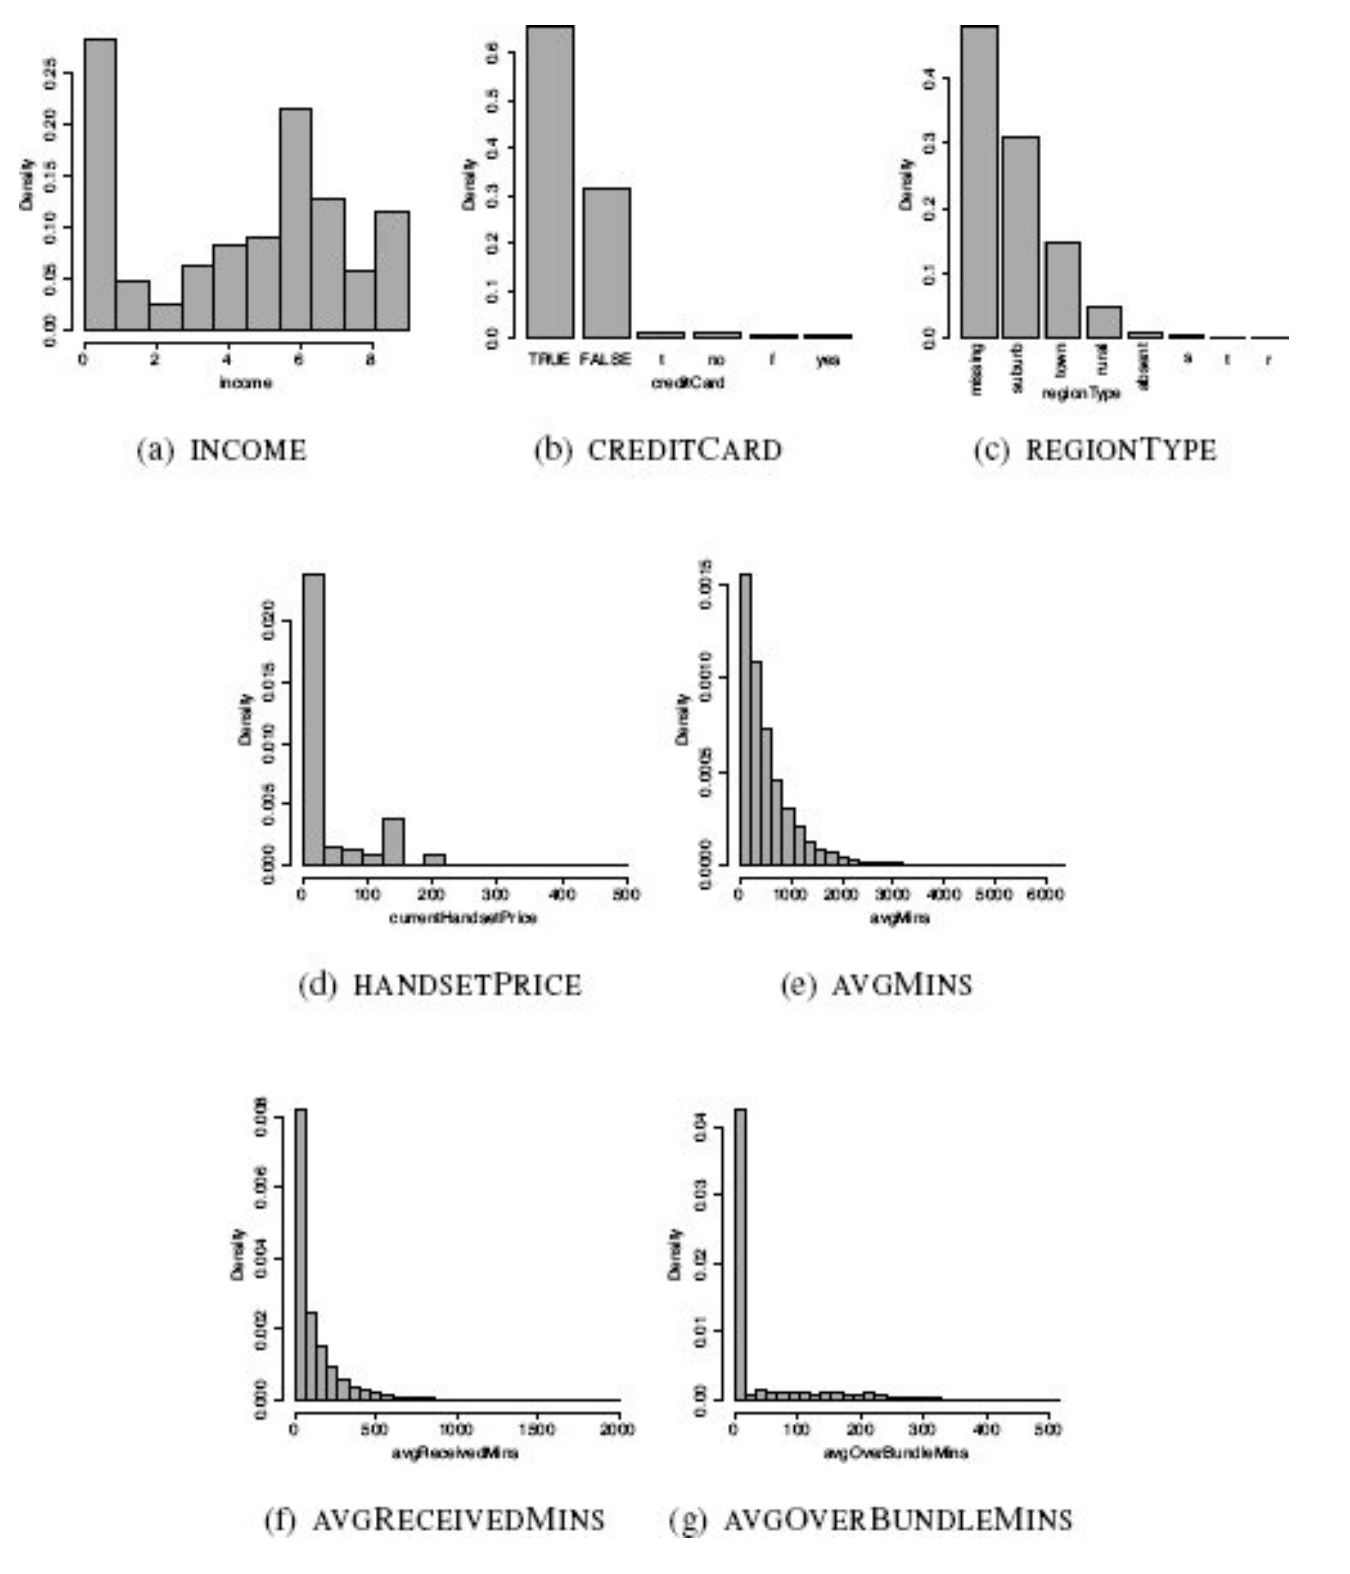
\includegraphics[scale=0.25]{images/first_figures.png}
\end{frame}

\begin{frame}{Data Quality Figures}
\centering
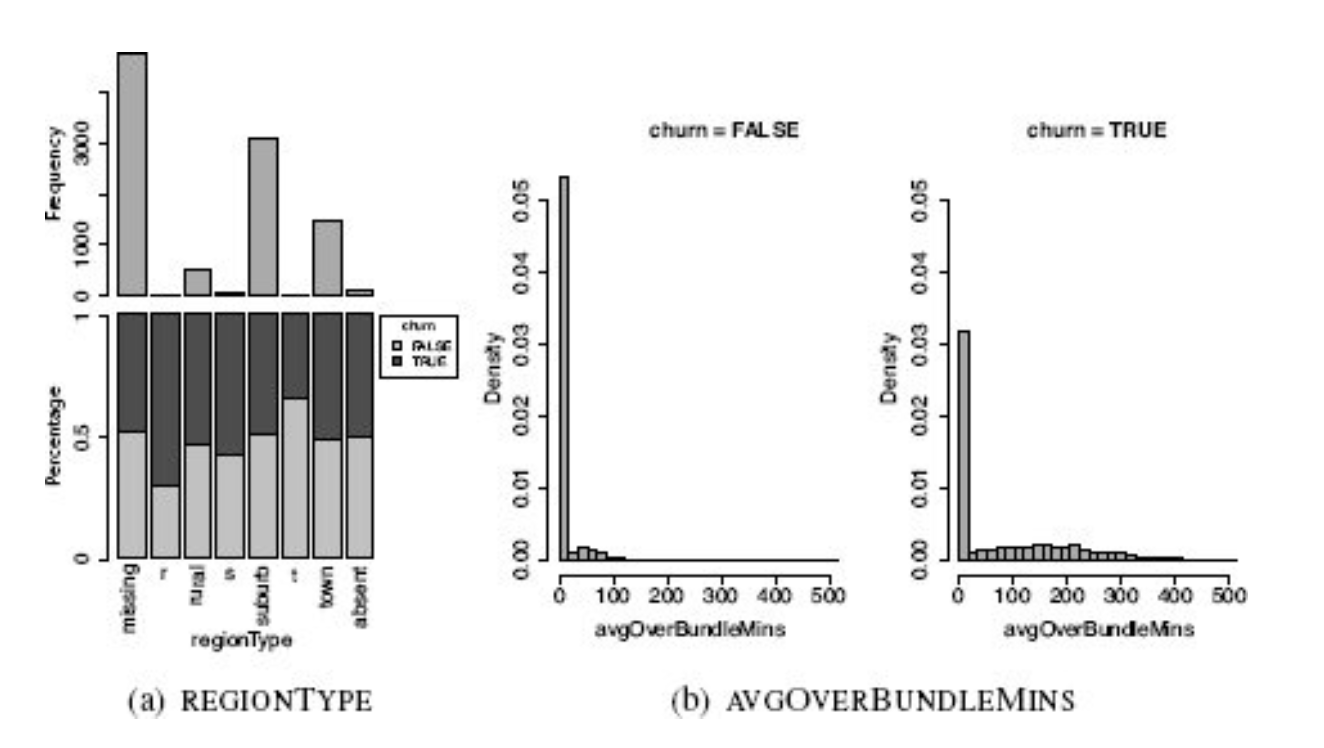
\includegraphics[scale=0.5]{images/second_figures.png}
\end{frame}

\begin{frame}{Data Quality Report}
\centering
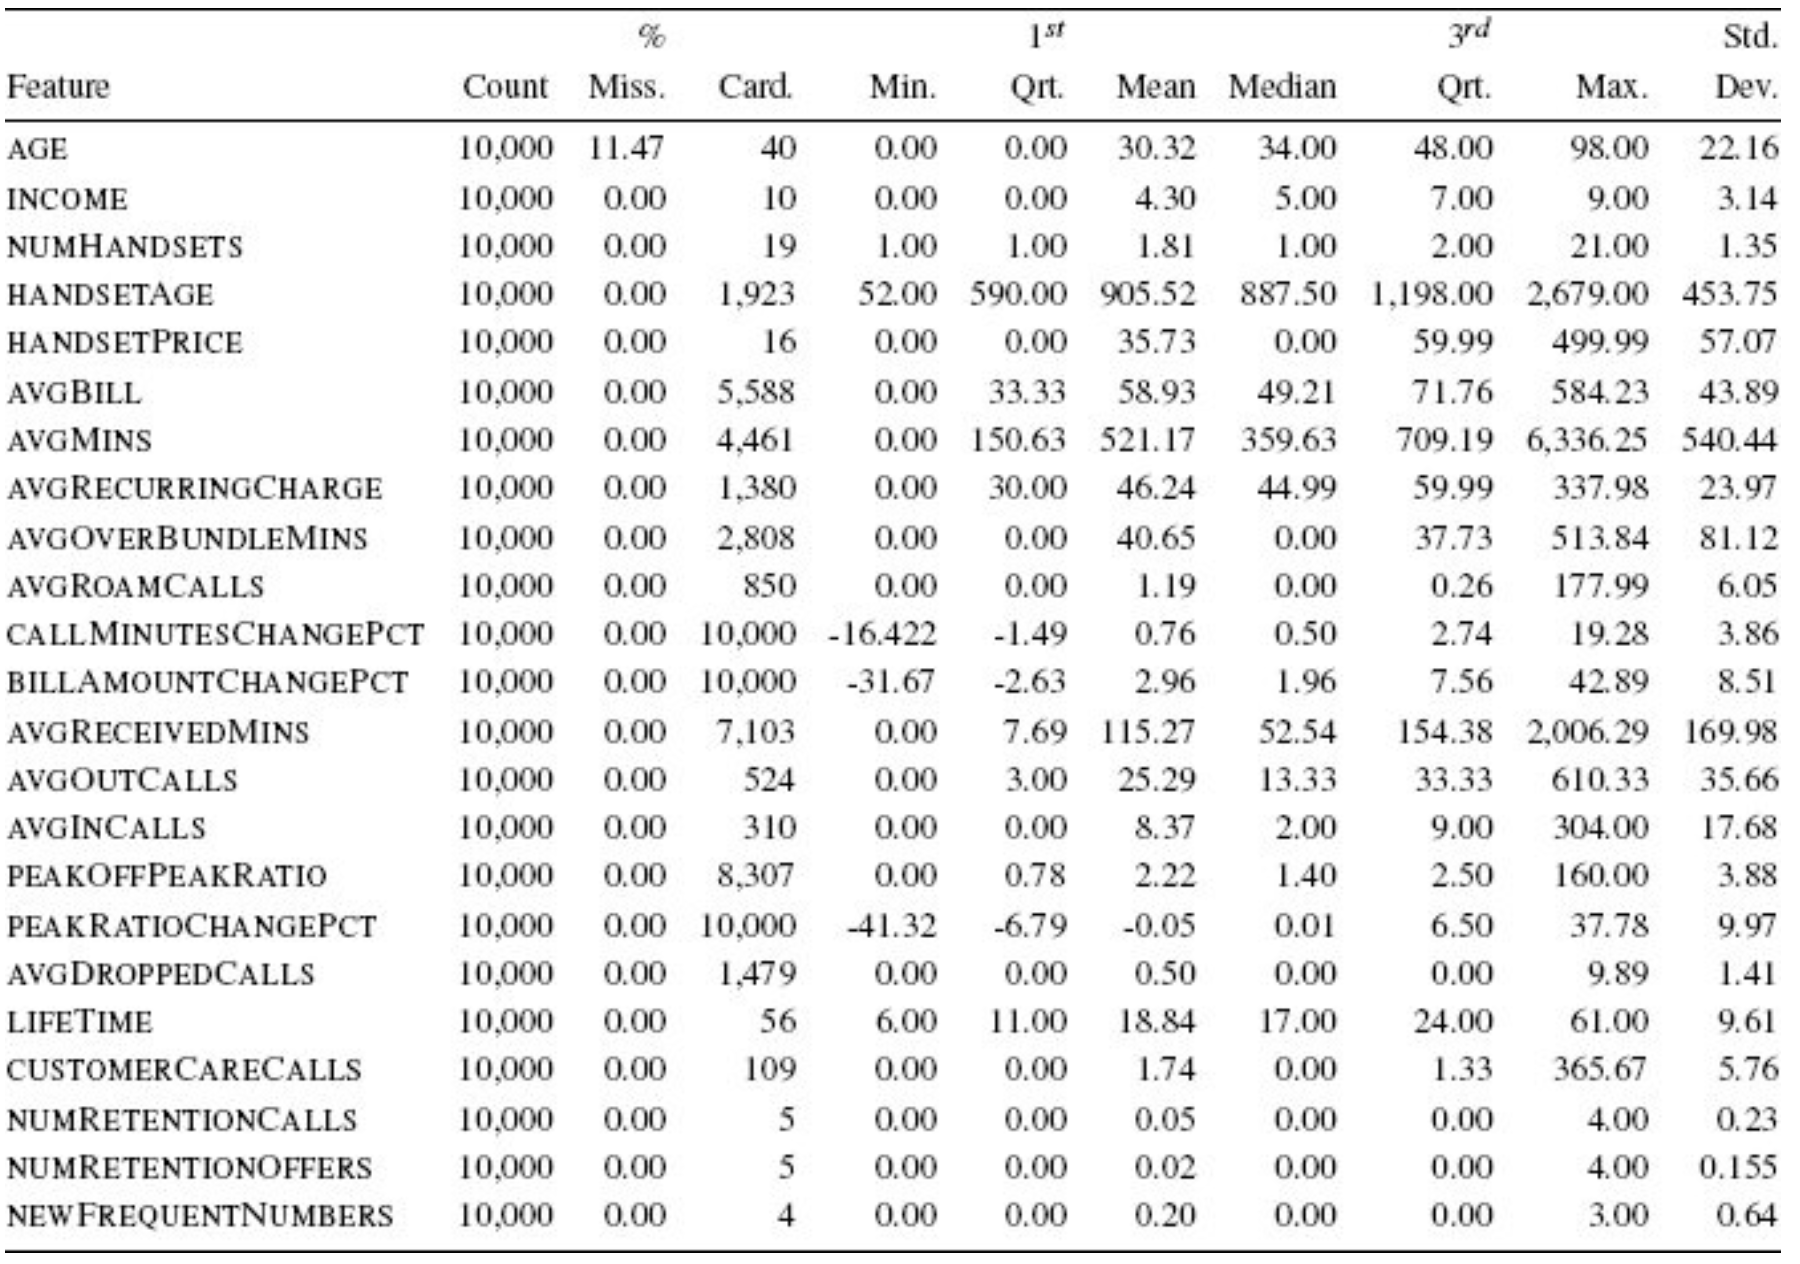
\includegraphics[scale=0.3]{images/data_qual_1.png}
\end{frame}

\begin{frame}{Data Quality Report}
\centering
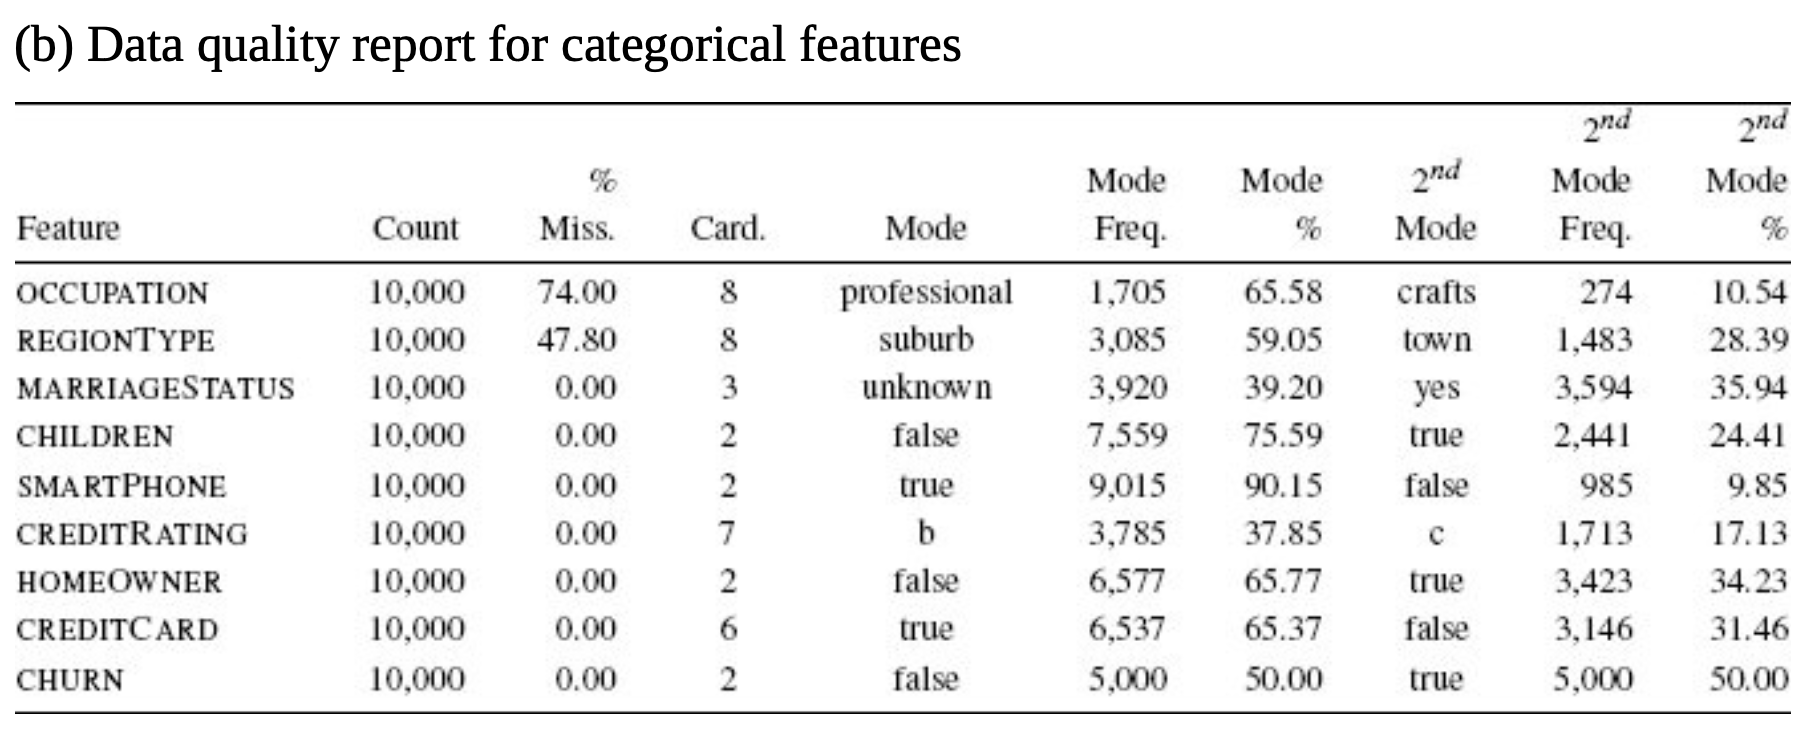
\includegraphics[scale=0.45]{images/data_qual_cat.png}
\end{frame}
%----------------------------------------------------------------------------------------

\begin{frame}{Choosing and Training the First Model}

\begin{itemize}
  \item The model needed to be:
  \begin{itemize}
    \item \textbf{Accurate}
    \item \textbf{Integrable} into A T's operational workflow
    \item \textbf{Interpretable}, to give insight into churn behavior
  \end{itemize}

  \item The ABT contained:
  \begin{itemize}
    \item A \textbf{categorical target feature} (churn vs. no churn)
    \item A mix of \textbf{continuous and categorical} descriptive features
  \end{itemize}

  \item \textbf{Decision trees} were selected due to:
  \begin{itemize}
    \item Compatibility with mixed data types
    \item Tolerance for missing values and outliers
    \item Easy interpretability and business alignment
  \end{itemize}

  \item Ross trained, tuned, and tested several decision trees:
  \begin{itemize}
    \item Used entropy-based information gain, binary splits, and no pruning
    \item Evaluation metric: \textbf{classification accuracy}
    \item Initial model achieved \textbf{74.87\% accuracy} on the hold-out test set
  \end{itemize}
\end{itemize}

\end{frame}

\begin{frame}{Unpruned, First Fit Tree}
\centering
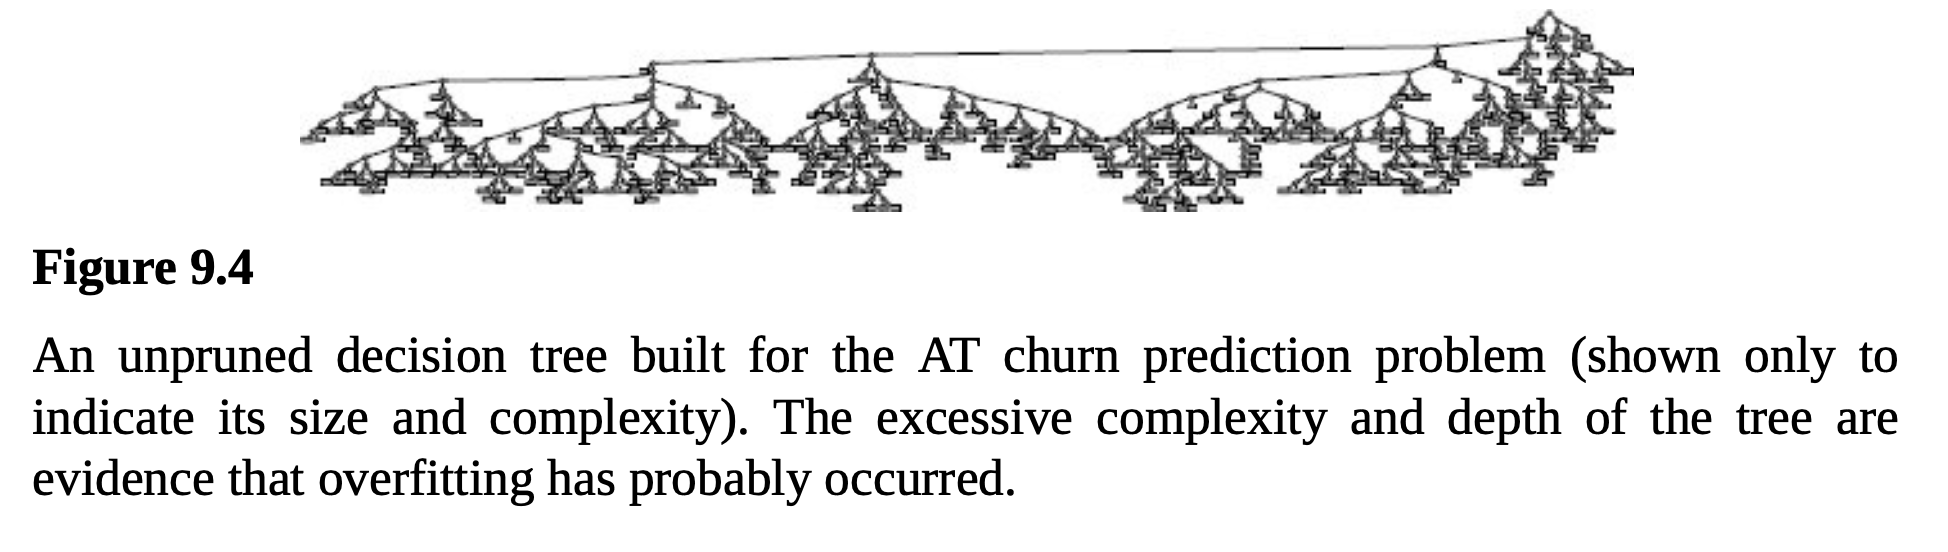
\includegraphics[scale=0.4]{images/unpruned.png}
\end{frame}


\begin{frame}{Pruned Decision Tree}
\centering
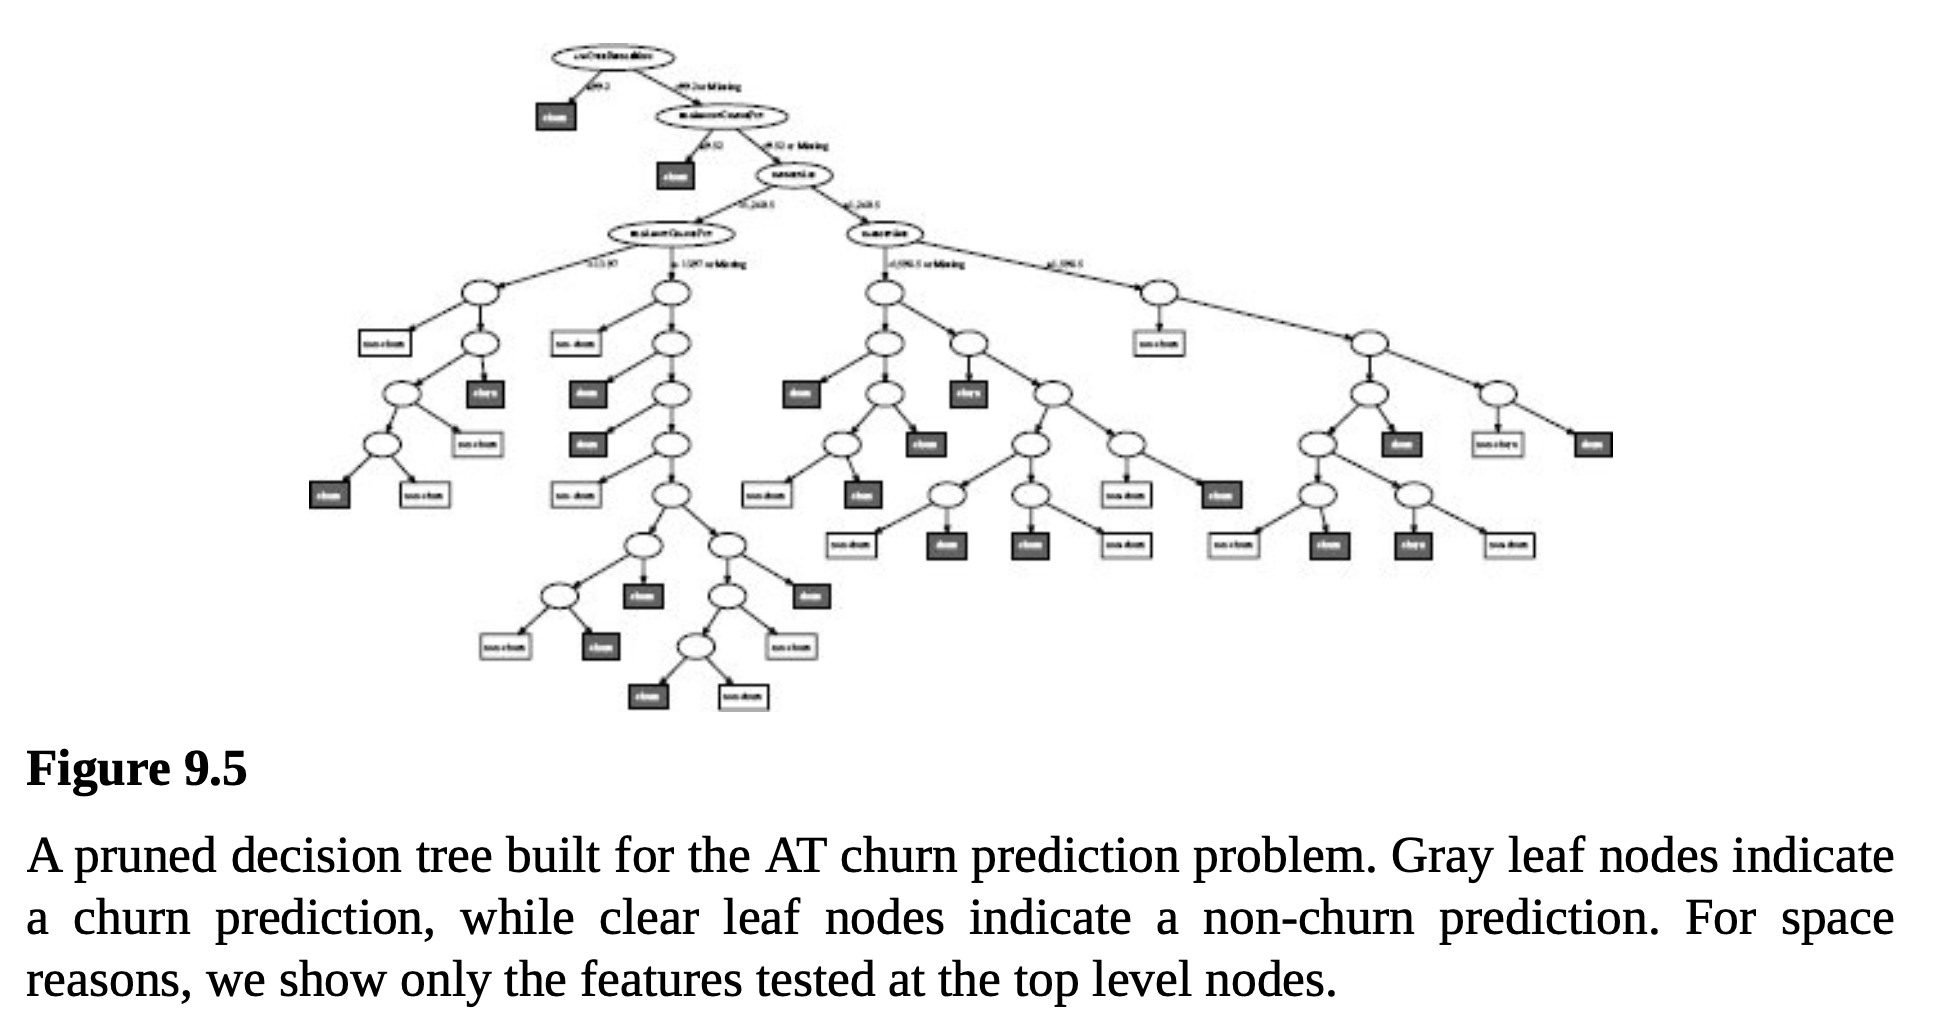
\includegraphics[scale=0.4]{images/pruned.png}
\end{frame}
%----------------------------------------------------------------------------------------

\begin{frame}{Confusion Matrix – Stratified Hold-Out Test Set}
Using pruning, Ross was able to increase the average class accuracy on the hold-out
test set to 79.03\%, a significant improvement over the previous model.
\begin{table}[ht]
\centering
\begin{tabular}{l|cc|c}
\textbf{Actual / Predicted} & \textbf{Churn} & \textbf{Non-Churn} & \textbf{Recall (\%)} \\
\hline
\textbf{Churn}      & 1,058 & 442   & 70.53 \\
\textbf{Non-Churn}  & 152   & 1,348 & 89.86 \\
\end{tabular}
\end{table}

\vspace{1em}
\textbf{Note:} This test set is \textbf{stratified}, meaning it preserves the same class balance (churn vs. non-churn) as the training set. This helps ensure fair and representative performance evaluation across both classes.
\begin{itemize}
  \item The model performs well across both classes.
  \item \textbf{Higher recall} for non-churners than churners - better for predicting non-churners.
\end{itemize}

\end{frame}

\begin{frame}{Confusion Matrix – Non-Stratified Hold-Out Test Set}

\begin{table}[ht]
\centering
\begin{tabular}{l|cc|c}
\textbf{Actual / Predicted} & \textbf{Churn} & \textbf{Non-Churn} & \textbf{Recall (\%)} \\
\hline
\textbf{Churn}      & 1,115 & 458    & 70.88 \\
\textbf{Non-Churn}  & 1,439 & 12,878 & 89.95 \\
\end{tabular}
\end{table}

\vspace{1em}
\begin{itemize}
  \item Results consistent with stratified test set.
  \item Slight improvement in recall for both classes.
  \item Indicates good generalization and model stability.
\end{itemize}

\end{frame}

\begin{frame}{Real-World Evaluation – Non-Stratified Test Set}

\begin{itemize}
  \item The initial \textbf{79.03\% accuracy} was based on a stratified test set (50:50 churn vs. non-churn).
  \item In reality, A T’s customer base is more like \textbf{10\% churners, 90\% non-churners}.
  \item To reflect this, Ross evaluated the model on a \textbf{non-stratified test set} with the true class distribution.
  \item Resulting \textbf{average class accuracy: 79.28\%}, still strong and consistent.
  \item Ross also used \textbf{cumulative gain and lift charts} to evaluate practical performance:
  \begin{itemize}
    \item The \textbf{cumulative gain chart} showed that contacting the top 40\% most at-risk customers would capture ~80\% of likely churners.
    \item This demonstrates the model's value in prioritizing retention efforts.
  \end{itemize}
\end{itemize}

\end{frame}

\begin{frame}{Pruned Decision Tree}
\centering
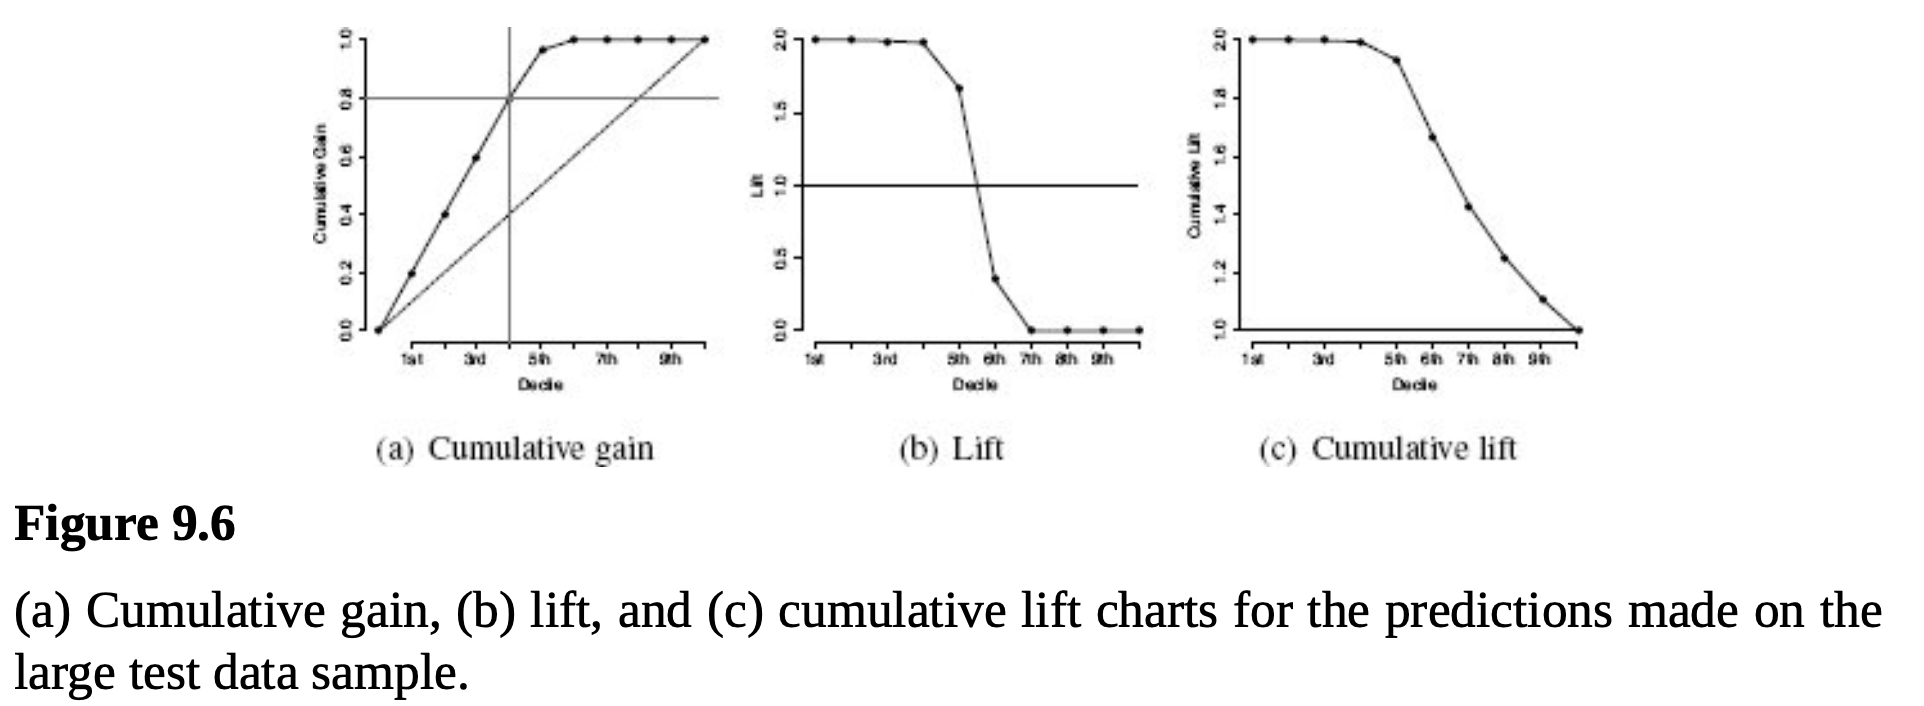
\includegraphics[scale=0.4]{images/eval_fig.png} \\

The cumulative gain chart shows that if A T were
to call just 40\% of their customer base, they would identify approximately 80\% of the
customers who are likely to churn, which is strong evidence that the model is doing a good
job of distinguishing between different customer types.
\end{frame}

\begin{frame}{Presenting the Model to the Business}

\begin{itemize}
  \item With strong performance established, Ross presented the model to broader business teams to build credibility and buy-in.
  \item For interpretability, he created a \textbf{stunted version of the decision tree}, limiting the depth to 5 levels.
  \begin{itemize}
    \item Full pruned tree was retained for deployment.
    \item Shallow trees highlight the most \textbf{informative and accessible splits}.
  \end{itemize}
  \item The simplified tree (next slide) revealed:
  \begin{itemize}
    \item \texttt{AVGOVERBUNDLEMINS}
    \item \texttt{BILLAMOUNTCHANGEPCT}
    \item \texttt{HANDSETAGE}
  \end{itemize}
  as key predictors of churn.
  \item These aligned well with customer behavior: unexpected billing changes, going over call bundles, or aging handsets may drive churn.
  \item Business stakeholders discussed why features like \texttt{CUSTOMERCARECALLS} (used in prior heuristics) were not selected—prompting broader insight.
\end{itemize}
\end{frame}

\begin{frame}{Pruned Decision Tree}
\centering
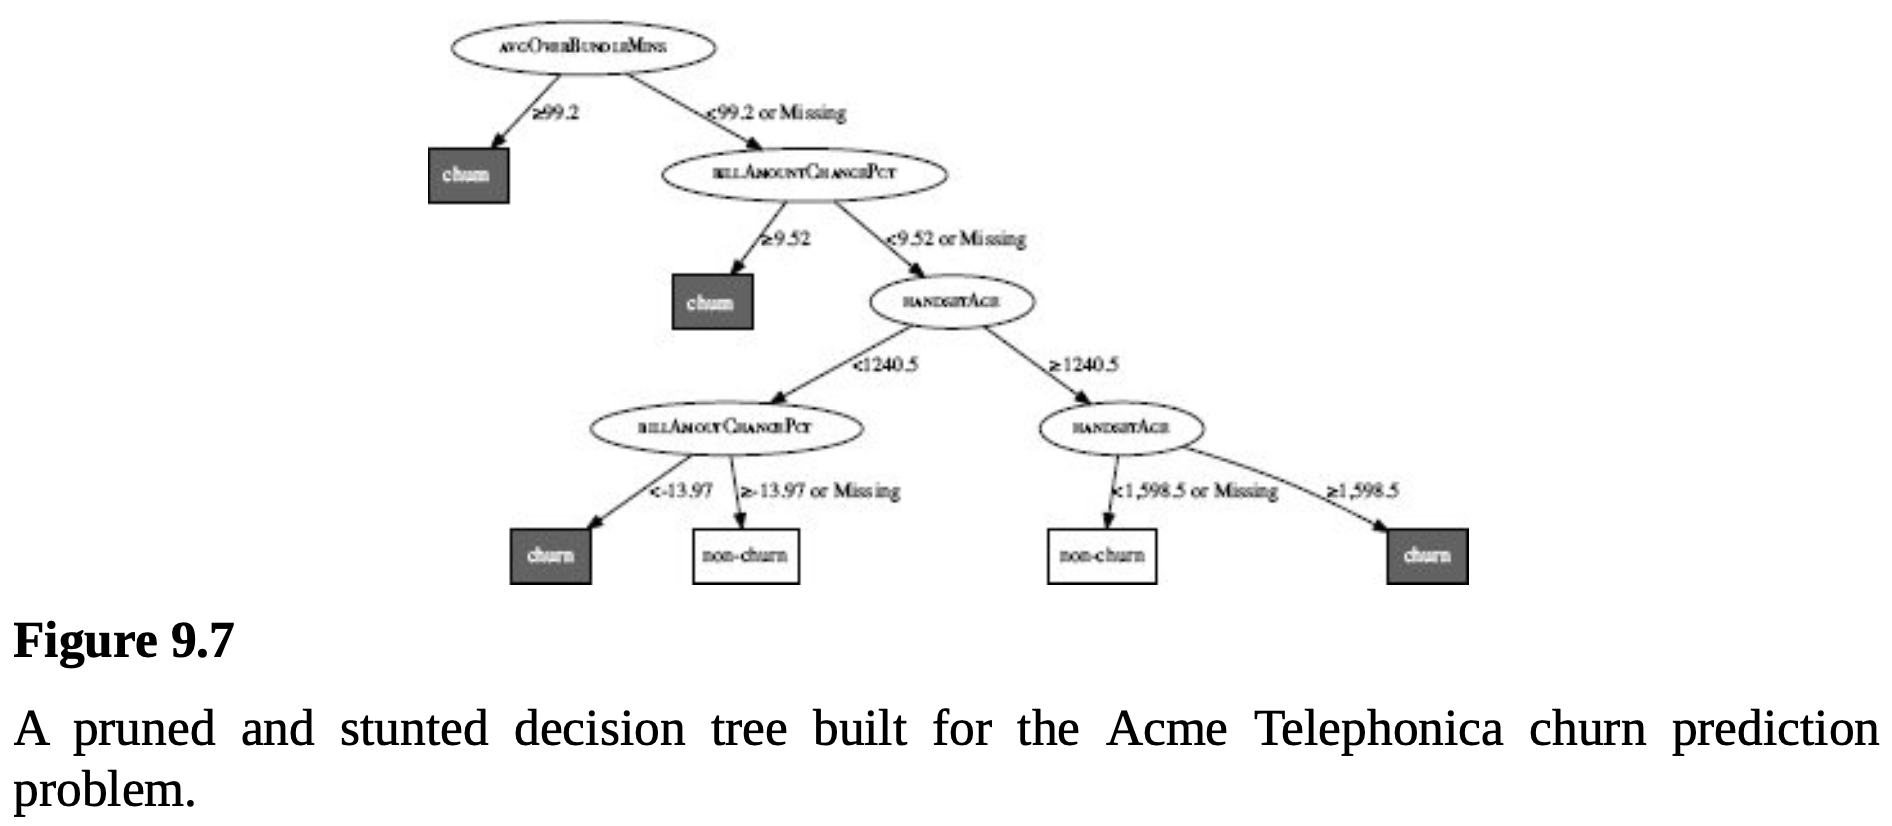
\includegraphics[scale=0.4]{images/stunted.png}
\end{frame}

\begin{frame}{Deployment and Model Monitoring}

\begin{itemize}
  \item Since A T already had a call list workflow, deploying the decision tree model was relatively straightforward.
  \item Key deployment tasks:
  \begin{itemize}
    \item \textbf{Revise data pipelines:} Returned to the Data Preparation phase to build robust ETL routines.
    \item \textbf{Integrate the model:} Code replaced the old rule-based system with the decision tree for generating retention call lists.
  \end{itemize}
  \item Ross worked with A T’s IT team to make the system reliable and repeatable on a monthly basis.
  \item To ensure long-term effectiveness, Ross implemented a \textbf{model monitoring system}:
  \begin{itemize}
    \item Quarterly reports evaluated prediction accuracy against observed churn (excluding contacted customers).
    \item If performance drifted significantly, the model was flagged as stale and retraining was triggered.
  \end{itemize}
\end{itemize}

\end{frame}

\end{document}